% MATEMÁTICAS PARA LA CIENCIA DE DATOS

\documentclass[
%xcolor={dvipsnames},
%hyperref={colorlinks},
%hyperref,
twoside,
12pt,
letterpaper, 
justified
%]{amsbook}
]{tufte-book}
%]{elegantbook}
%,graybox,envcountchap,sectrefs]{svmono}
\usepackage{fontenc}
\usepackage{graphicx}
\usepackage[utf8]{inputenc}
\usepackage[spanish,mexico]{babel}
\usepackage{fontenc}
\usepackage{amsmath}
\usepackage{amssymb}
\usepackage{graphicx}
\usepackage{mathrsfs}
\usepackage{yfonts}
\usepackage{enumerate}
\usepackage{mathtools}
\usepackage{textcomp}
\usepackage{lmodern}
\usepackage{fancyvrb}
\usepackage{multicol}
\usepackage{wrapfig}
\usepackage{floatflt}
\usepackage{filecontents}
\usepackage{hyperref}
%\usepackage{bibentry}
\usepackage{graphicx} % Allows including images
\usepackage{booktabs} % Allows the use of \toprule,
\usepackage{mdframed}
\usepackage[dvipsnames]{xcolor}
\usepackage{tikz}
\usepackage{amsthm}
\usepackage{hyperref}
\usepackage{listings}
\usepackage{units}
\usepackage{color}
%\newenvironment{solucion}{\begin{proof}[Solución]}\begin{color}{red}\end{color}{\end{proof}}

\usetikzlibrary{matrix,arrows,decorations.pathmorphing}
 
\hypersetup{
	pdftitle={Estadística Matemática},
	pdfauthor={Juliho Castillo Colmenares},
	colorlinks=true	
%	linkcolor=BrickRed,
%	filecolor=BrickRed,
%	citecolor = BrickRed,      
%	urlcolor=BrickRed,
	%frenchlinks=true
}


% add numbers to chapters, sections, subsections
\setcounter{tocdepth}{1}
\setcounter{secnumdepth}{1}

% chapter format
\titleformat{\chapter}%
{\huge\rmfamily\itshape\color{BrickRed}}% format applied to label+text
{\llap{\colorbox{BrickRed}{\parbox{1.5cm}{\hfill\itshape\huge\color{white}\thechapter}}}}% label
{2pt}% horizontal separation between label and title body
{}% before the title body
[]% after the title body

% section format
\titleformat{\section}%
{\normalfont\Large\itshape\color{BrickRed}}% format applied to label+text
{\llap{\colorbox{BrickRed}{\parbox{1.5cm}{\hfill\color{white}\thesection}}}}% label
{1em}% horizontal separation between label and title body
{}% before the title body
[]% after the title body

% subsection format
\titleformat{\subsection}%
{\normalfont\large\itshape\color{BrickRed}}% format applied to label+text
{\llap{\colorbox{BrickRed}{\parbox{1.5cm}{\hfill\color{white}\thesubsection}}}}% label
{1em}% horizontal separation between label and title body
{}% before the title body
[]% after the title body
%%% MANDATORY!!!

\newcommand{\R}{\mathbb{R}}
\newcommand{\N}{\mathbb{N}}
\newcommand{\Q}{\mathbb{Q}}
\newcommand{\C}{\mathbb{C}}
\newcommand{\Z}{\mathbb{Z}}

\newcommand{\set}[1]{\left\{ #1 \right\}}
\newcommand{\evat}[2]{\left. #1 \right|_{#2}}
\newcommand{\sett}[2]{\left\{ \left.#1 \right| #2 \right\} }

\newcommand{\inp}[1]{\langle #1 \rangle}
\newcommand{\norm}[1]{\left\| #1 \right\|}
\newcommand{\abs}[1]{\left|#1\right|}
\newcommand{\imply}{\rightarrow}

%precalculo

\newcommand{\mcd}{mcd}
\newcommand{\mcm}{mcm}

% Calculo
\newcommand{\del}{\delta}
\renewcommand{\a}{\alpha}
\newcommand{\Del}{\Delta}
\newcommand{\sech}{sech}
\newcommand{\csch}{csch}
\newcommand{\ep}{\epsilon}
\newcommand{\p}{\partial}

%ecuaciones diferenciales
\newcommand{\lap}[1]{\mathcal{L}\set{#1}}
\newcommand{\lapin}[1]{\mathcal{L}^{-1}\set{#1}}
\newcommand{\lam}{\lambda}

%álgebra lineal

\renewcommand{\a}{\alpha}
\renewcommand{\b}{\beta}

\newcommand{\gen}[1]{\operatorname{gen}\left( #1 \right)}

\newcommand{\av}{\arrowvert}

\newcommand{\id}{\operatorname{Id}}

\newcommand{\im}{\mathfrak{I}}

\renewcommand{\Im}{\operatorname{Im}}

\newcommand{\nul}[1]{\operatorname{nul}\left( #1 \right)}
\newcommand{\ran}[1]{\operatorname{ran}\left( #1 \right)}

\newcommand{\ssi}{\Leftrightarrow}
\newcommand{\basis}[1]{\left( #1 \right)}
\renewcommand{\th}{\theta}
\renewcommand{\arg}[1]{\varphi(#1)}
\newcommand{\bm}[1]{\begin{bmatrix}#1\end{bmatrix}}
% add numbers to chapters, sections, subsections
\setcounter{tocdepth}{1}
\setcounter{secnumdepth}{1}

\theoremstyle{theorem}
\newtheorem{teorema}{Teorema}[chapter]
\newtheorem{lema}{Lema}[chapter]
\newtheorem{proposicion}{Proposición}[chapter]
\newtheorem*{corolario}{Corolario}%[chapter]
%\newtheorem*{algoritmo}{Algoritmo}%[chapter]

\theoremstyle{definition}
\newtheorem{problema}{Problema}[chapter]
\newtheorem{ejemplo}{Ejemplo}[chapter]
\newtheorem*{definicion}{Definición}%[chapter]
\newtheorem*{axioma}{Axioma}%[chapter]
\newtheorem*{propiedad}{Propiedad}%[chapter]
%\newtheorem{ejemplo}{Ejemplo}[chapter]

\theoremstyle{remark}
\newtheorem*{observacion}{Observación}%[chapter]
\newtheorem*{sugerencia}{Sugerencia}

\newenvironment{solucion}{
	\medskip
	%\begin{framed}
		\bgroup\color{Maroon}
		{\textbf{Solución.}}
	}{
		\egroup
	%\end{framed}
	\medskip
	}

%\newenvironment{ejemplo}{
%	\medskip
%	%\begin{framed}
%	\bgroup\color{RedOrange}
%	{\textbf{Ejemplo.}}
%}{
%	\egroup
%	%\end{framed}
%	\medskip
%}

\newenvironment{algoritmo}[1]{
	\medskip
	%\begin{framed}
	\bgroup
	\color{RedViolet}
	{\textbf{Algoritmo. (#1)}}
	\ttfamily
}{
	\egroup
	%\end{framed}
	\medskip
}
\newcommand{\f}{\phi}
\newcommand{\vphi}{\varphi}
\newcommand{\vf}{\varphi}
\newcommand{\flow}[2]{\varphi^{#1}\left( #2 \right)}
\renewcommand{\d}[1]{\dot{#1}}
\renewcommand{\r}{\rho}
\newcommand{\A}{\mathcal{A}}
\newcommand{\gam}{\gamma}
\renewcommand{\a}{\alpha}
\renewcommand{\b}{\beta}
\newcommand{\om}{\omega}
\newcommand{\iso}{\simeq}
\newcommand{\tensor}{\otimes}
\newcommand{\inc}{\hookrightarrow}
\renewcommand{\L}{\mathcal{L}}
\renewcommand{\H}{\mathcal{H}}
\newcommand{\D}{\mathcal{D}}
\newcommand{\converge}[1]{\xrightarrow{#1}}
\newcommand{\cott}[1]{T^{*}\T^{#1}}
%\newcommand{\G}{\mathcal{G}}
\newcommand{\hu}{\textbf{h}}
\newcommand{\deck}[1]{\operatorname{Dake}\left( #1 \right)}
\newcommand{\til}[1]{\tilde{#1}}
\newcommand{\Gam}{\Gamma}
\newcommand{\grad}{\nabla}
\newcommand{\var}{\Delta}
\newcommand{\avch}[2]{\frac{\Delta #1}{\Delta #2}}
\newcommand{\Avch}[2]{\dfrac{\Delta #1}{\Delta #2}}
\newcommand{\Err}{\operatorname{Err}}
\newcommand{\wed}{\wedge}
\newcommand{\biconditional}{\longleftrightarrow}
\newcommand{\yields}{\vdash}
\newcommand{\onlyif}{\Rightarrow}
\newcommand{\uset}{\mathbb{U}}
\newcommand{\minus}{\backslash}
\newcommand{\symdif}{\oplus}
\newcommand{\rel}[1]{{ {\color{blue}\textbf{#1}} }}
\newcommand{\dominio}[1]{\operatorname{Dominio}\left( #1 \right)}
\newcommand{\imagen}[1]{\operatorname{Imagen}\left( #1 \right)}
\newcommand{\nrel}[1]{{ {\color{red}\not}{\color{orange}\textbf{#1}} }}
\newcommand{\comp}[2]{#1 \circ #2}

\theoremstyle{definition}
  \newtheorem{conj}{Conjectura}[chapter]
%  \newtheorem{prob}{Problema}[chapter]
  \newtheorem*{ax}{Axioma}
  \newtheorem{tdv}{Tabla de Verdad}

\theoremstyle{remark}
  \newtheorem{claim}{Afirmación}[chapter]
  %\newtheorem{rem}{Observación}[chapter]
  %\newtheorem*{note}{Nota}
  \newtheorem{case}{Caso}


\renewcommand{\d}[1]{\dot{#1}}
\renewcommand{\r}{\rho}
\renewcommand{\a}{\alpha}
\renewcommand{\b}{\beta}
\renewcommand{\L}{\mathcal{L}}
\renewcommand{\H}{\mathcal{H}}

\newcommand{\Var}{\operatorname{Var}}
\newcommand{\s}{\sigma}
\newcommand{\comb}[2]{\begin{pmatrix} #1 \\ #2\end{pmatrix}}
\newcommand{\cov}{\operatorname{Cov}}


\title{}
\author[J. Colmenares]{Juliho Colmenares}
\publisher{www.asimovian.academy\\math.vader@yahoo.com}


\usepackage{units}

\begin{document}
	\maketitle
	\tableofcontents

\chapter{Probabilidad}

\input{pe-01 Probabilidad Básica}
\chapter{Variables Aleatorias Discretas}


Supongamos que a cada punto del espacio muestral se le asigna un número.  Entonces hemos definido una \emph{función} en el espacio muestral  Esta función es llamada \emph{variable aleatoria} (o \emph{variable estocástica}) o de manera más precisa \emph{función aleatoria}. 


Usualmente, las variables aleatorias se denotan por letras mayúsculas como $X$ o $Y$. En general, una variable aleatoria tiene algún significado físico, geométrico, económico, financieros, etc.


[t]
\begin{ejemplo}
  \label{exmp:2.1}
Supongamos que una moneda se lanza dos veces de manera que el espacio muestral es $\set{HH,HT,TH,TT}.$  Digamos que $X$ representa el número de soles ($H$) que obtenemos.
\end{ejemplo}


\section{Funciones de probabilidad discretas}

 Sea $X$ una variable aleatoria discreta.  Supongamos que los valores que puede tomar son $x_{1},...,x_{k},$ arreglados en algún orden dado.  Supongamos también que esos valores
 tienen alguna probabilidad dada por
 \begin{align}
 \label{2.1}
 	P(X=x_{k})=f(x_{k}).
 \end{align}


{Función de probabilidad}
\begin{align}
\label{2.2}
P(X=x)=
\begin{cases}
f(x) & x=x_{k} \\
0	& \text{en otro caso}
\end{cases}
\end{align}



	En general, $f(x)$ será una función de probabilidad si
	\begin{align*}
		\begin{cases}
			f(x)\geq 0 \\
			\sum_{x}f(x)=1.
		\end{cases}
	\end{align*}



	\begin{ejemplo}
		\label{exmp:2.2}
		Encuentre la función de probabilidad correspondiente a la variable aleatoria $X$ del ejemplo \ref{exmp:2.1}.
	\end{ejemplo}



 \begin{ejemplo}
  \label{sol:2.1}
  Suponga que un par de dados se lanzan. Sea $X$ la variable aleatoria dada por la suma de los puntos. Encuentre la distribución de probabilidad de $X.$
 \end{ejemplo}



 \begin{ejemplo}
  \label{sol:2.2}
  Encuentre la distribución de probabilidad de niños y niñas en familias con 3 hijos, suponiendo la misma probabilidad para niños y niñas.
 \end{ejemplo}



\section{Funciones de distribución para variables aleatorias discretas}


	La función de distribución de una variable discreta $X$ se obtiene de la función de probabilidad a través de la siguiente fórmula
	\begin{align}
		\label{2.4}
		F(x) = P(X\leq x) = \sum_{u \leq x} f(u).
	\end{align}



	Si $X$ toma sólo un número finito de valores $x_{1},...,x_{n}$ entonces la función de distribución está dada por
	\begin{align}
		\label{2.5}
		F(x)=
		\begin{cases}
			0 & -\infty < x < 0 \\
			f(x_{1}) & x_{1} \leq x < x_{2} \\
			f(x_{1})+f(x_{2}) & x_{2} \leq x < x_{3} \\
			\vdots & \vdots \\
			f(x_{1})+\cdots+f(x_{n}) & x_{n} \leq x < \infty
		\end{cases}
	\end{align}



	\begin{ejemplo}
		\label{exmp:2.3}
		Encuentre la función de distribución para la variable aleatoria $X$ del ejemplo \ref{exmp:2.2} y obtenga su gráfica.
	\end{ejemplo}



	\begin{figure}
	\centering
	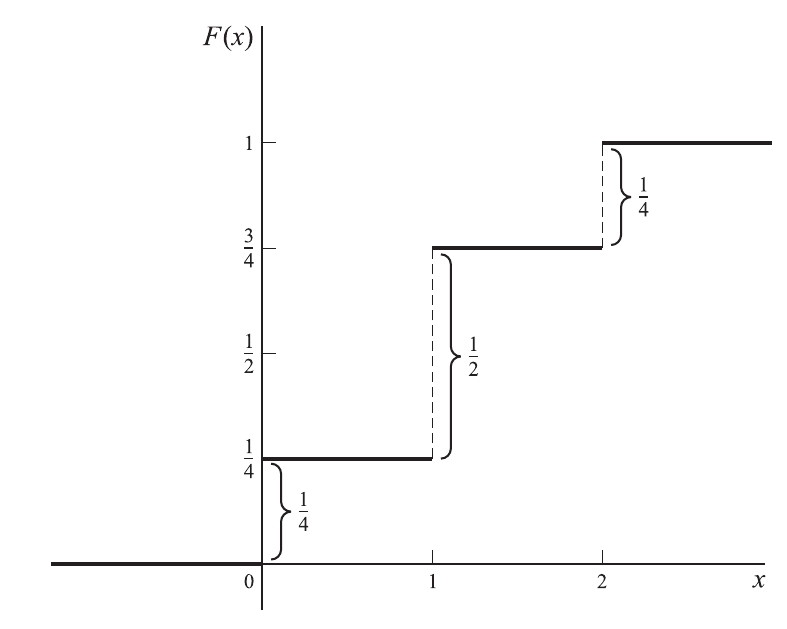
\includegraphics[height=7cm,keepaspectratio=true]{./pe/pands0201.png}
	% pands0201.png: 0x0 pixel, 300dpi, 0.00x0.00 cm, bb=
	\label{fig:0201}
\end{figure}



	\begin{rem}
		\begin{itemize}
			\item Los saltos en la función de distribución están determinados por el valor de la función de probabilidad. 
			\item Este tipo de funciones se conoce como \emph{función escalonada}.  Debe observarse que son \emph{continuas por la derecha.}
			\item La función de distribución es \emph{monótonamente creciente.}
		\end{itemize}

	\end{rem}



	La función de probabilidad se puede obtener a partir de la función de distribución con la siguiente fórmula
	\begin{align}
		\label{2.6}
		f(x)=F(x)-\lim_{u \to x^{-}}F(u).
	\end{align}



 \begin{ejemplo}
  \label{sol:2.3}
  \begin{enumerate}[(a)]
   \item Encuentre la función de distribución $F(x)$ para la variable aleatoria del problema resuelto \ref{sol:2.1};
   \item grafique esta función de distribución.
  \end{enumerate}

 \end{ejemplo}



 \begin{figure}[h]
 \centering
 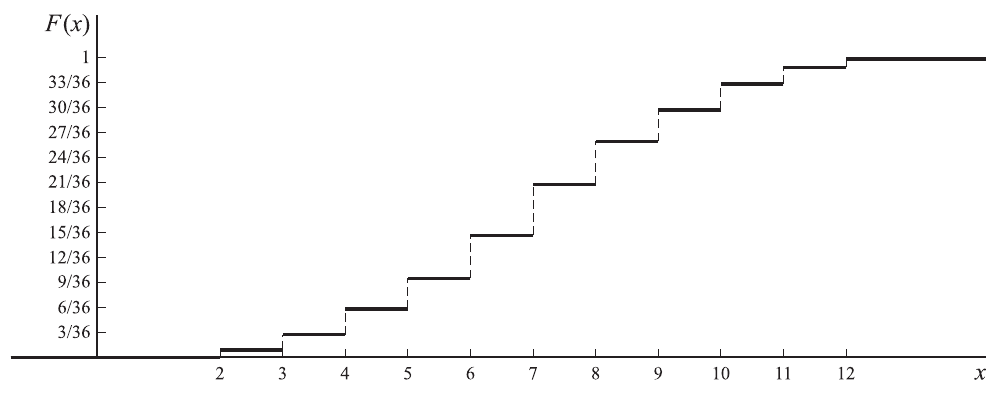
\includegraphics[width=10cm,keepaspectratio=true]{./pe/pands0206.png}
 % pands0206.png: 0x0 pixel, 300dpi, 0.00x0.00 cm, bb=
\end{figure}




 \begin{ejemplo}
  \label{sol:2.4}
  \begin{enumerate}[(a)]
   \item Encuentre la función de distribución $F(x)$ para la variable aleatoria del problema resuelto \ref{sol:2.2};
   \item grafique esta función de distribución.
  \end{enumerate}

 \end{ejemplo}



 \begin{figure}[h]
 \centering
 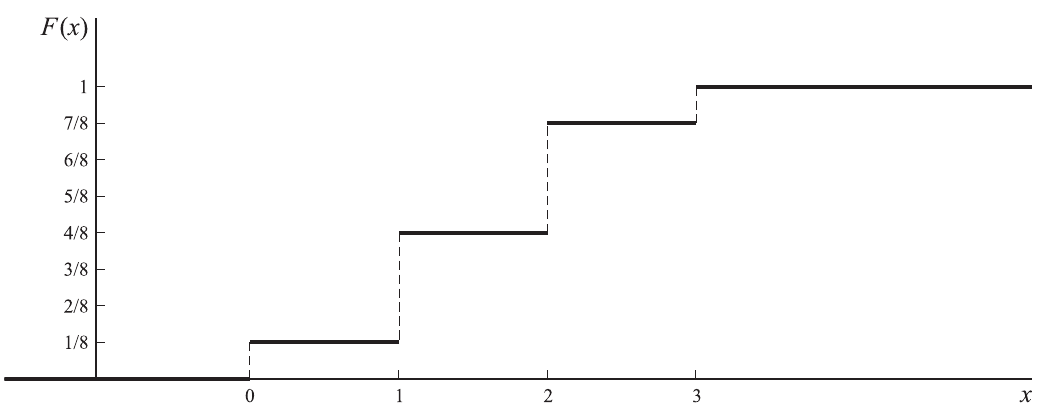
\includegraphics[width=10cm,keepaspectratio=true]{./pe/pands0207.png}
 % pands0206.png: 0x0 pixel, 300dpi, 0.00x0.00 cm, bb=
\end{figure}


\chapter{Variable Aleatorias Continuas}

	Una variable aleatoria no discreta $X$ se llama \emph{absolutamente continua} (o simplemente \emph{continua}) si su función de distribución puede ser representada como
	\begin{align}
		 \label{2.7}
		 F(x)=P(X \leq x)=\int_{-\infty}^{x} f(u)du, \; -\infty < x <\infty.
	\end{align}


	La función $f$ usualmente se llama \emph{densidad de probabilidad} y debe satisfacer las siguientes propiedades:
	\begin{enumerate}
		\item $f(x)\geq 0 $
		\item $\displaystyle \int_{-\infty}^{\infty}f(x)dx=1.$
	\end{enumerate}




	La probabilidad de que $X$ se encuentre entre dos valores $a$ y $b$ está dada por
	\begin{align}
		\label{2.8}
		P(a < x <b)=\int_{a}^{b}f(x)dx.
	\end{align}


[t]
	\begin{align}
		\label{exmp:2.4}
		P(X=a)=0.
	\end{align}


Por tanto, en \eqref{2.8} podemos reemplazar cualquier signo $<$ por $\leq.$

[t]
	\begin{ejemplo}
		\label{exmp:2.5}
		\begin{enumerate}[(a)]
			\item Encuentre la constante $c$ tal que la función
			\begin{align}
				f(x)=
				\begin{cases}
					cx^{2} & 0 < x < 3 \\
					0 & \texttt{en otro caso}
				\end{cases}
			\end{align}
			sea una función de probabilidad. 
			\item Calcule $P(1 < X < 2).$
		\end{enumerate}

	\end{ejemplo}


[t]
	\begin{ejemplo}
	  \label{exmp:2.6}
	  Encuentre la distribución de probabilidad para la variable aleatoria del ejemplo
	  \ref{exmp:2.5} y utilícela para calcular $P(1 < x \leq 2).$
	\end{ejemplo}



	La probabilidad de que $X$ se encuentre entre $x$ y $x+\Del x$ esta dada por
	\begin{align}
		\label{2.9}
		P(x \leq X \leq x+\Del x)= \int_{x}^{x+\Del x}f(u)du,
	\end{align} 
	de manera que si $\Del x \approx 0,$ tendremos que
	\begin{align}
		\label{2.10}
		P(x \leq X \leq x+\Del x)\approx f(x) \Del x.
	\end{align}



	También podemos deducir de \eqref{2.7}, al diferenciar de ambos lados, que
	\begin{align}
		\label{2.11}
		\dfrac{dF(x)}{dx} = f(x)
	\end{align}
en todos aquellos puntos en que $f(x)$ sea continua.  Es decir, la derivada de la función de distribución es la función de densidad.


	\begin{rem}
		Existen variables aleatorias que no son discretas ni continuas.  Por ejemplo
		\begin{align}
			F(x)=
			\begin{cases}
				0 & x <1 \\
				\frac{x}{2} & 1 \leq x < 2 \\
				1 & x \leq 2.
			\end{cases}
		\end{align}

	\end{rem}



 \begin{ejemplo}
  \label{sol:2.5} Una variable aleatoria $X$ tiene función de densidad
  \begin{align}
   f(x)=\dfrac{c}{x^{2}+1}, \; -\infty < x <\infty.
  \end{align}

  \begin{enumerate}[(a)]
   \item Encuentre el valor de $c$; 
   \item encuentre la probabilidad de que
   \begin{align*}
    \dfrac{1}{3}< X^{2} <1.
   \end{align*}

  \end{enumerate}

 \end{ejemplo}



 \begin{ejemplo}
  \label{sol:2.6}
  Encuentre la función de distribución correspondiente a la función de densidad del problema resuelto \ref{sol:2.5}
 \end{ejemplo}



 \begin{ejemplo}
  \label{sol:2.7}
  La función de distribución para una variable aleatoria $X$ es
  \begin{align}
   F(x)=
   \begin{cases}
    1-e^{-2x} & x\geq 0 \\
    0 & x <0
   \end{cases}
  \end{align}

  Encuentre
  \begin{enumerate}[(a)]
   \item la función de densidad;
   \item la probabilidad de que $X>2$;
   \item la probabilidad que $-3 < X \leq 4.$
  \end{enumerate}


 \end{ejemplo}



\section{Interpretación gráfica}


	La distribución $F(x)=P(X\leq x)$ es monótonamente creciente de $0$ a $1...$
	\begin{figure}[h]
	\centering
	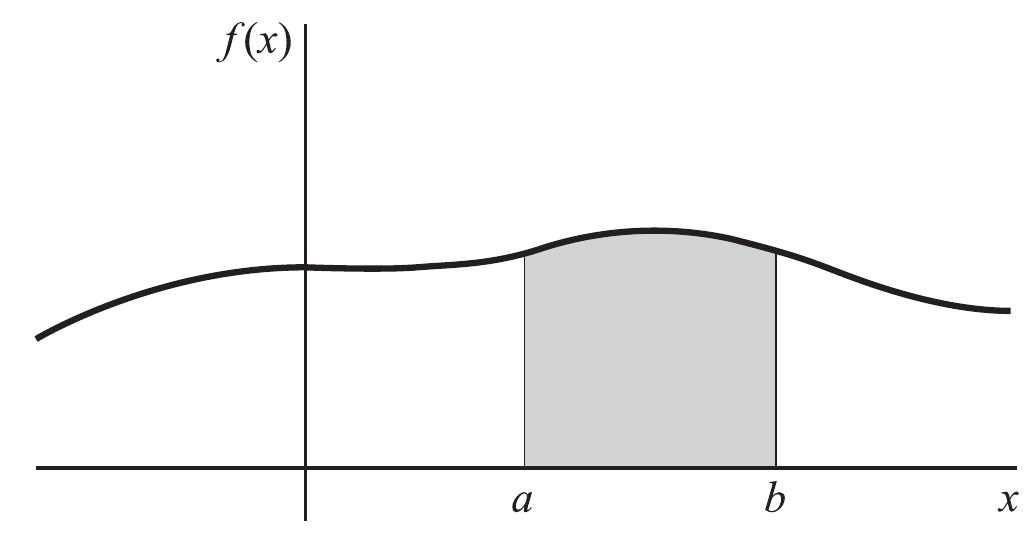
\includegraphics[height=5cm,keepaspectratio=true]{./pe/pands0202.png}
	% pands0202.png: 0x0 pixel, 300dpi, 0.00x0.00 cm, bb=
\end{figure}




  ...y el área bajo dicha curva es igual a $1.$
  \begin{figure}[h]
	\centering
	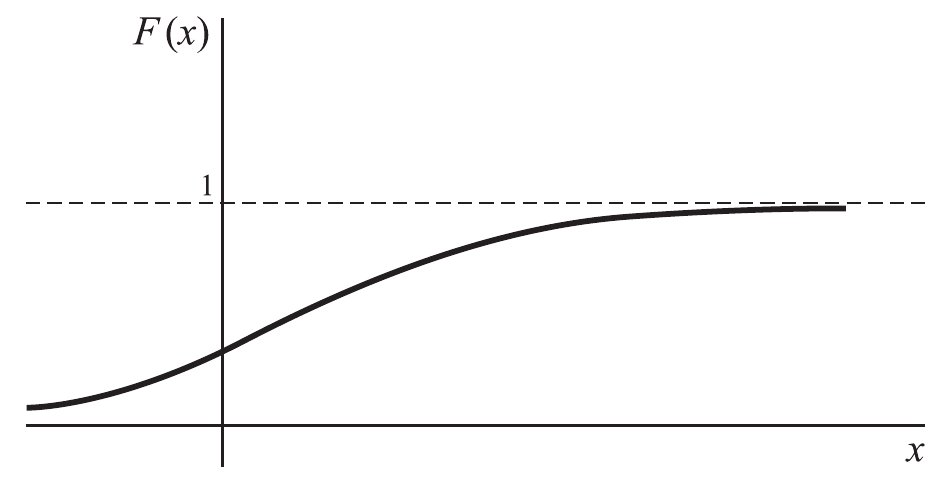
\includegraphics[height=5cm,keepaspectratio=true]{./pe/pands0203.png}
	% pands0203.png: 0x0 pixel, 300dpi, 0.00x0.00 cm, bb=
\end{figure}




\section{Distribución conjunta de probabilidad}


	Las ideas anteriores se generalizan fácilmente a dos o más variables.


{Caso discreto}
	Si $X$ y $Y$ son ambas variables aleatorias discretas, definimos la \emph{función de probabilidad conjunta} de $X$ y $Y$ por
	\begin{align}
	\label{2.13}
		P(X=x, Y=y)=f(x,y)
	\end{align}
 donde
\begin{enumerate}
	\item $f(x,y)\leq 0;$
	\item $\sum_{k}\sum_{y}f(x,y)=1.$
\end{enumerate}




	Supongamos que $X$ sólo toma uno de los $m$ valores $x_{1},...,x_{m},$ mientras que $Y$ tomas sólo toma uno de los $n$ valores $y_{1},...,y_{n}.$

	Entonces la probabilidad del evento $X=x_{j}, Y=y_{k}$ está dada por
	\begin{align}
	\label{2.14}
		P(X=x_{j}, Y=y_{k})=f(x_{j},y_{k})
	\end{align}



	Una función de probabilidad conjunta para $X$ y $Y$ puede ser representada por una \emph{tabla de probabilidad conjunta} como la siguiente:
	\begin{figure}[h]
	\centering
	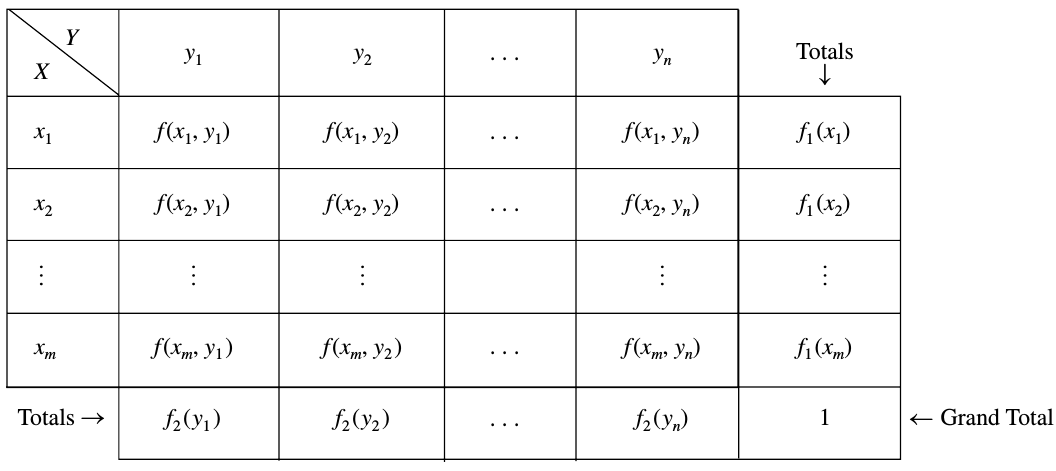
\includegraphics[height=5cm,keepaspectratio=true]{./pe/tab0203.png}
	% tab0203.png: 0x0 pixel, 300dpi, 0.00x0.00 cm, bb=
	\label{tab:0203}
\end{figure}



	La probabilidad de $X=x_{j}$ se obtiene de la siguiente manera
	\begin{align}
	\label{2.15}
		P(X=x_{j})=f_{X}(x_{j})=\sum_{k=1}^{n}f(x_{j},y_{k}).
	\end{align}



	De manera similar, la probabilidad de $Y=y_{k}$ se obtiene de la siguiente manera
	\begin{align}
	\label{2.16}
		P(Y=y_{k})=f_{Y}(y_{k})=\sum_{j=1}^{m}f(x_{j},y_{k}).
	\end{align}


 
 	Nos referiremos a $f_{X}(x)$ y $f_{Y}(y)$ como \emph{funciones de probabilidad marginal} de $X$ y $Y$ respectivamente.
 

	Observe que
	\begin{align}
	\label{2.17}
		\sum_{j=1}^{m}f_{X}(x_{j})=1,
		\sum_{k=1}^{n}f_{Y}(y_{k})=1,
	\end{align}
	lo cual se puede reescribir como
	\begin{align}
		\label{2.18}
		\sum_{j=1}^{m}\sum_{k=1}^{n}f(x_{j},y_{k})=1.
	\end{align}



	La \emph{función de distribución conjunta } está definida por
	\begin{align}
	\label{2.19}
		F(x,y)=P(X\leq x, Y\leq y)
		=\sum_{u\leq x}\sum_{v\leq y}f(u,v)
	\end{align}



{Caso continuo}
	El caso en el que ambas variables son continuas es obtenido de manera análoga reemplazando las sumas por integrales.


	La \emph{función de probabilidad conjunta} (o de manera más común \emph{función de densidad conjunta}) de $X$y $Y$ está definida por
	\begin{enumerate}
		\item $f(x,y)\geq 0;$
		\item $\displaystyle \int_{-\infty}^{\infty}\int_{-\infty}^{\infty}
		f(x,y) dxdy=1.$
	\end{enumerate}



	Gráficamente $z=f(x,y)$ representa una \emph{superficie de probabilidad}
\begin{figure}[h]
	\centering
	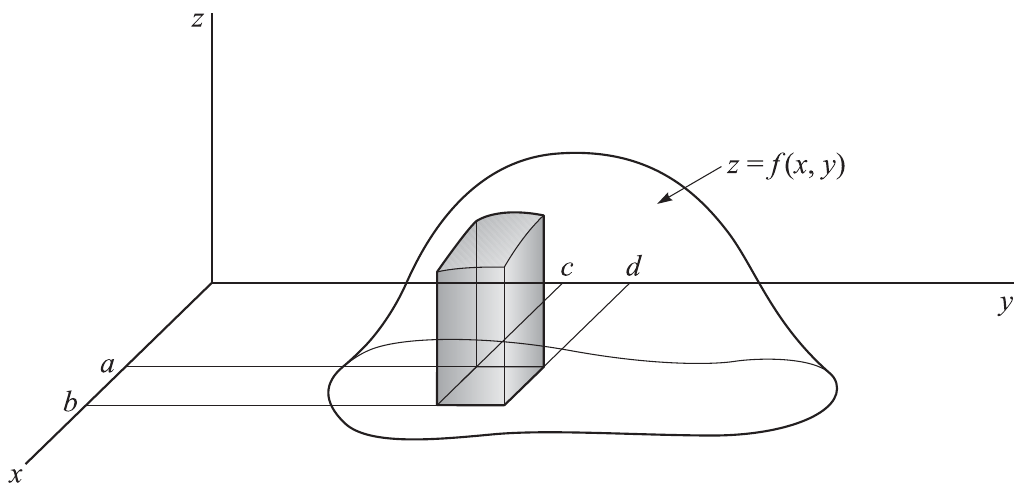
\includegraphics[height=3cm,keepaspectratio=true]{./pe/pands0204.png}
	% pands0204.png: 0x0 pixel, 300dpi, 0.00x0.00 cm, bb=
	\label{fig:2.4}
\end{figure}
tal que el volumen bajo la superficie es igual a $1.$


	\begin{align}
		\label{2.20}
		P(a<X<b,c<Y<d)=\int_{a}^{b}\int_{c}^{d}f(x,y)dydx.
	\end{align}



	A cada evento $A$ corresponde una región $\mathcal{R}_{A}$ del plano $xy$ tal que
	\begin{align}
	  \label{2.21}
		P(A)=\iint_{\mathcal{R}_{A}}f(x,y)dxdy.
	\end{align}



	La \emph{función de distribución conjunta} de $X$ y $Y$ en este caso está definida por
	\begin{align}
		\label{2.22}
	F(x,y)=P(X\leq x, Y\leq y)=
	\int_{-\infty}^{x} \int_{-\infty}^{y} f(u,v)dvdu.
	\end{align}



	Se sigue que
	\begin{align}
	 \dfrac{\partial^{2}F}{\partial x \partial y}=
	 f(x,y)  \label{2.23} \\
	  	 P(X\leq x)=F_{X}(x)=\int_{-\infty}^{x}\int_{-\infty}^{\infty} f(u,v)dvdu \label{2.24} \\
	 	 P(Y\leq y)=F_{Y}(y)=\int_{-\infty}^{\infty}\int_{-\infty}^{y} f(u,v)dvdu \label{2.25}
	\end{align}



 Diremos que $F_{X}(x),F_{Y}(y)$ son las \emph{funciones de distribución marginal,} o simplemente \emph{funciones distribuciones,} de $X$ y $Y$, respectivamente.


 Las derivadas de \eqref{2.24} y \eqref{2.25} con respecto a $x$ y $y$ son llamadas \emph{funciones de densidad marginal}, o simplemente las \emph{funciones de densidad,} de $X$ y $Y$ están dados por
 \begin{align}
 \label{2.26}
 \displaystyle
  f_{X}(x)=\int_{-\infty}^{\infty}f(x,v)dv, \;
  f_{Y}(x)=\int_{-\infty}^{\infty}f(u,y)du.
 \end{align}



\section{Variables Aleatorias Independientes}

 Supongamos que $X$ y $Y$ son variables aleatorias discretas.  Si los eventos $X=x$ y $Y=y$ son eventos independientes para todo $x,y,$  entonces diremos que $X,Y$ son v.a's independientes.


 En tal caso,
 \begin{align}
  \label{2.27}
  P(X=x,Y=y)=P(X=x)P(Y=y),
 \end{align}
o de manera equivalente
\begin{align}
 f(x,y)=f_{X}(x)f_{Y}(y).
\end{align}



 De manera inversa, si para todo $x,y$ la función de probabilidad conjunta $f(x,y)$ pueden ser expresada como el producto de funciones de probabilidad marginal $f_{X}(x)f_{Y}(y),$ entonces $X,Y$ son independientes.
 

 Si no pueden expresarse de dicha manera, entonces $X,Y$ son dependientes.


 Si $X,Y$ son v.a's continuas, diremos que son \emph{independientes} si los eventos $X\leq x$ y $Y\leq y$ son independientes para todo $x,y.$

 En tal caso, escribiremos
 \begin{align}
  \label{2.29}
  P(X\leq x, Y \leq y)=P(X\leq x)P(Y\leq y)
 \end{align} 
 o de manera equivalente
 \begin{align}
  F(x,y)=F_{X}(x)F_{Y}(y)
 \end{align}
 donde $F_{X}(x)$ y $F_{Y}(y)$ son las funciones de distribución marginal de $X,Y$ respectivamente.



 De manera inversa, si para todo $x,y$ la función de probabilidad conjunta $f(x,y)$ pueden ser expresada como el producto de funciones de probabilidad marginal $F_{X}(x)F_{Y}(y),$ entonces $X,Y$ son independientes.
 

 Si no pueden expresarse de dicha manera, entonces $X,Y$ son dependientes.


 Para v.a's independientes continuas, también es cierto que la función de densidad conjunta $f(x,y)$ es el producto de funciones $f_{X}(x)f_{Y}(y)$ y estas son las funciones de densidad marginal de $X,Y$ respectivamente.



 \begin{ejemplo}
  \label{sol:2.8}
  La función de probabilidad conjunta de dos variables discretas $X,Y$ está dada por
  \begin{align}
   f(x,y)=
   \begin{cases}
    c(2x+y) & 0\leq x \leq 2, \; 0 \leq y \leq 3 \\
    0 & \texttt{en otro caso}.
   \end{cases}
  \end{align}
  \begin{enumerate}[(a)]
   \item Encuentre el valor de la constante $c;$
   \item encuentre $P(X=2,Y=1);$
   \item encuentre $P(X\geq 1, Y\leq 2).$
  \end{enumerate}

 \end{ejemplo}



 \begin{figure}[h]
 \centering
 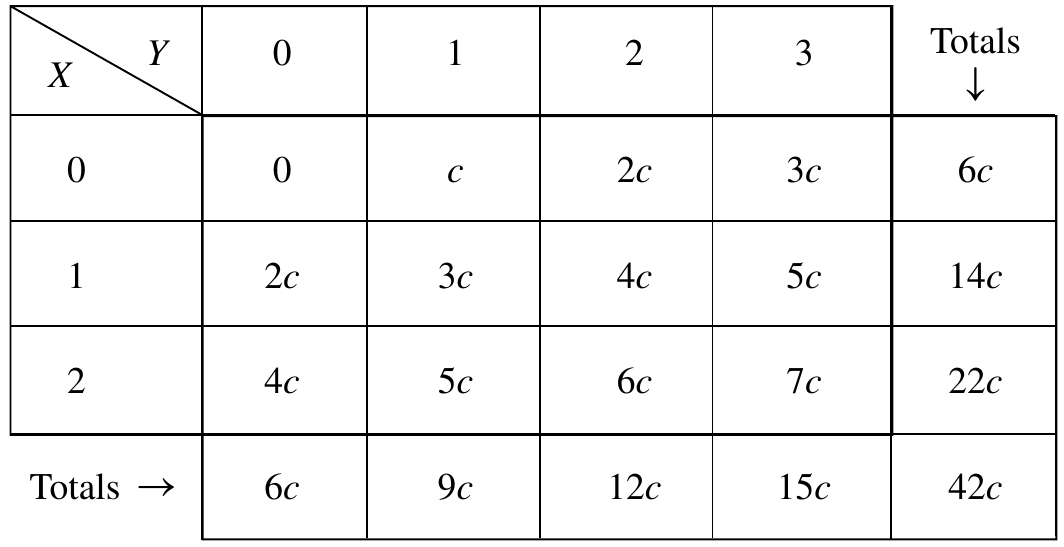
\includegraphics[width=10cm,keepaspectratio=true]{./pe/tab0206.png}
 % tab0206.png: 0x0 pixel, 300dpi, 0.00x0.00 cm, bb=
 \label{tab:2.6}
\end{figure}



 \begin{ejemplo}
  \label{sol:2.9}
  Encuentre las funciones de probabilidad marginal para $X$ y $Y$ en el problema resuelto \ref{sol:2.8}.
 \end{ejemplo}



 \begin{ejemplo}
  \label{sol:2.10}
  Muestre que las variables aleatorias del problema resuelto \ref{sol:2.8} son dependientes.
 \end{ejemplo}



 \begin{ejemplo}
  \label{sol:2.11}
  La función de densidad conjunta de dos variables aleatorias continuas $X$ y $Y$ es
  \begin{align}
   f(x,y)=
   \begin{cases}
    cxy & 0<x<4, \; 1<y<5\\
    0 & \texttt{en otro caso}.
   \end{cases}
  \end{align}

 \end{ejemplo}
\begin{enumerate}[(a)]
 \item Encuentre el valor de $c$;
 \item encuentre $P(1<X<2,2<Y<3)$;
 \item encuentre $P(X\geq 3, Y\leq 2)$.
\end{enumerate}



 \begin{ejemplo}
  \label{sol:2.12}
  Encuentre las funciones de probabilidad marginal de las v.a's $X,Y$ del problema resuelto \ref{sol:2.11}.
 \end{ejemplo}



 \begin{ejemplo}
  \label{sol:2.13}
  Encuentre la función de distribución conjunta para las v.a's del problema resuelto \ref{sol:2.11}.
 \end{ejemplo}



 \begin{center}
 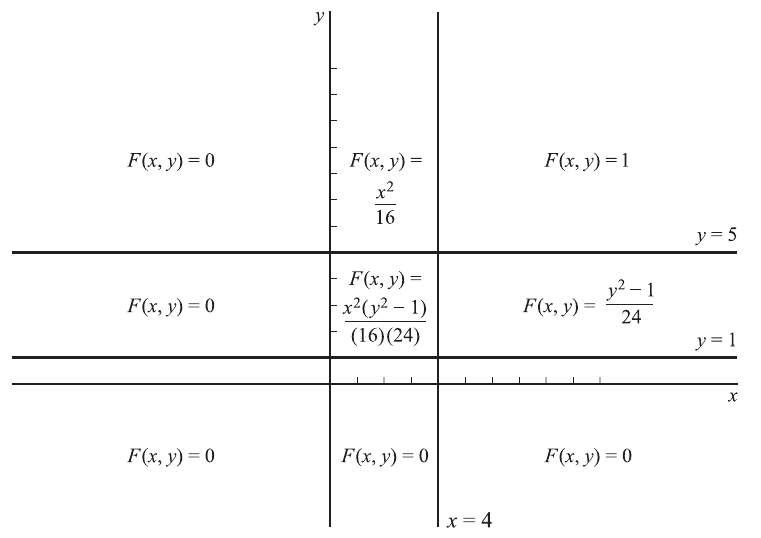
\includegraphics[width=10cm,keepaspectratio=true]{./pe/pands0209.png}
 % pands0209.png: 0x0 pixel, 300dpi, 0.00x0.00 cm, bb=
\end{center}




 \begin{ejemplo}
  \label{sol:2.14}
  En el problema resuelto \ref{sol:2.11}, encuentre $P(X+Y<3)$.
 \end{ejemplo}



 \begin{center}
 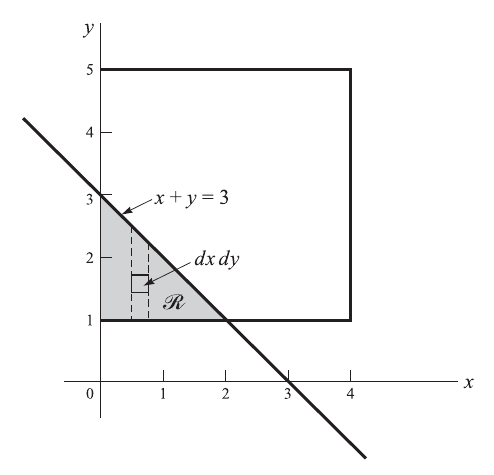
\includegraphics[height=8cm,keepaspectratio=true]{./pe/pands0210.png}
 % pands0210.png: 0x0 pixel, 300dpi, 0.00x0.00 cm, bb=
\end{center}



\section{Distribución Condicional}

 Nosotros ya sabemos que si $P(A)>0,$
 \begin{align}
  \label{2.41}
  P(B|A)=\dfrac{P(A\cap B)}{P(A)}.
 \end{align}



 Si $X,Y$ son v.a's discretas y tenemos los eventos $A=\set{X=x}, \; B=\set{Y=y},$ entonces \eqref{2.41} se convierte
 \begin{align}
  \label{2.42}
  P(Y=y|X=x)=
  \begin{cases}
   \dfrac{f(x,y)}{f_{X}(x)} & 0 < f_{X}(x)  \\
   0 & \texttt{en otro caso}
  \end{cases}
 \end{align}
 $f(x,y)=P(X=x,Y=y)$ es la función de probabilidad conjunta, mientras que $f_{X}(x)$ es la función de probabilidad marginal para $X.$


 Definimos la \emph{función de probabilidad condicional de $Y$ dado $X$} como
 \begin{align}
  \label{2.43}
  f(y|x)=
  \begin{cases}
   \dfrac{f(x,y)}{f_{X}(x)} & 0 < f_{X}(x)  \\
   0 & \texttt{en otro caso}
  \end{cases}
 \end{align}



 De manera similar, definimos la \emph{función de probabilidad condicional de $X$ dado $Y$} como
 \begin{align}
  \label{2.44}
  f(x|y)=
  \begin{cases}
   \dfrac{f(x,y)}{f_{Y}(y)} & 0 < f_{Y}(y)  \\
   0 & \texttt{en otro caso}
  \end{cases}
 \end{align}


 Estas ideas son fácilmente extensibles al caso donde $X,Y$ son v.a's continuas.


 Por ejemplo, la \emph{función de densidad condicional de $Y$ dado $X$} es
 \begin{align}
  \label{2.45}
  f(y|x)=
    \begin{cases}
   \dfrac{f(x,y)}{f_{X}(x)} & 0 < f_{X}(x)  \\
   0 & \texttt{en otro caso}
  \end{cases}
 \end{align}
 donde $f(x,y)$ es la función de densidad conjunta de $X$ y $Y$ y $f_{X}(x)$ es la función de densidad marginal de $X.$


 Usando \eqref{2.45} podemos por ejemplo encontrar que la probabilidad que $Y$  se encuentre entre $c$ y $d$ dado que $X=x$ es
 \begin{align}
  \label{2.46}P(c<Y<d|X=x)=
  \int_{c}^{d}f(y|x)dy.
 \end{align}




 \begin{ejemplo}
  \label{sol:2.27}
  Para la distribución del problema resuelto \ref{sol:2.8}, encuentre
  \begin{enumerate}[(a)]
   \item $f(y|2)$; y  
   \item $P(Y=1|X=2)$
  \end{enumerate}

 \end{ejemplo}



\begin{ejemplo}
 \label{sol:2.28}
  Si $X$ y $Y$ tienen función de densidad conjunta
 \begin{align}
  f(x,y)=
  \begin{cases}
   \frac{3}{4}+xy & 0<x<1, \; 0<y<1 \\
   0 & \texttt{en otro caso},
  \end{cases}
 \end{align}
encuentre
\begin{enumerate}[(a)]
 \item $f(y|x)$; 
 \item $P(Y>\frac{1}{2}| X = \frac{1}{2} )$.
\end{enumerate}

\end{ejemplo}



 \begin{ejemplo}
  \label{sol:2.29}
  La función de densidad conjunta de las variables aleatorias $X$ y $Y$ está dada por
  \begin{align}
   f(x,y)=
   \begin{cases}
    8xy & 0\leq x \leq 1, 0\leq y \leq x \\
    0 & \texttt{en otro caso}.
   \end{cases}
  \end{align}
Encuentre
\begin{enumerate}[(a)]
 \item la densidad marginal de $X$; 
 \item la densidad marginal de $Y$; 
 \item la densidad condicional de $X$; 
 \item la densidad condicional de $Y$.
\end{enumerate}

 \end{ejemplo}



 \begin{center}
 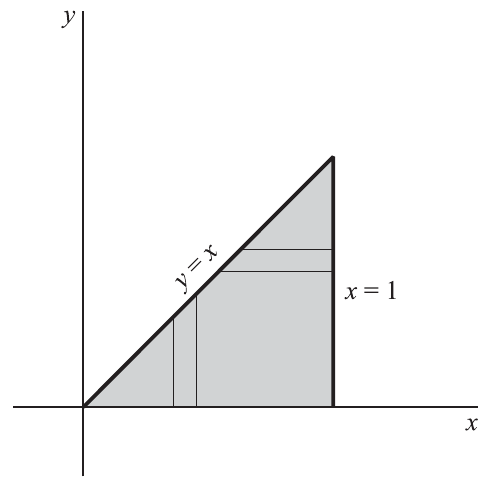
\includegraphics[height=7cm,keepaspectratio=true]{./pe/pands0217.png}
 % pands0217.png: 0x0 pixel, 300dpi, 0.00x0.00 cm, bb=
\end{center}



 \begin{ejemplo}
  \label{sol:2.30}
  Determine si las v.a's del problema resuelto \ref{sol:2.29} son independientes.
 \end{ejemplo}



\input{pe-03 Esperanza Matemática}
\chapter{Distribuciones especiales}


\section{La Distribución Binomial}


 Si $p$ es la probabilidad de que en un solo ensayo ocurra un evento (llamada la probabilidad de éxito) y $q = 1 - p$ es la
probabilidad de que este evento no ocurra en un solo ensayo (llamada probabilidad de fracaso), entonces la probabilidad de que el evento ocurra exactamente $x$ veces en $N$ ensayos (es decir, que ocurran $x$ éxitos y $N - x$ fracasos) está
dada por
\begin{align}
 \label{eq:7.1}
 f(x)=P(X=x)=\comb{N}{x}p^{x}q^{N-x}
\end{align}
donde $x=0,1,...,N.$


 \begin{ejemplo}
  \label{exmp:7.1}
  La probabilidad de obtener exactamente dos caras en seis lanzamientos de una moneda es
  \begin{align}
   \comb{6}{2}\left( \dfrac{1}{2} \right)^{2}\left( \dfrac{1}{2} \right)^{6-2}=\dfrac{15}{64}
  \end{align}
empleando \eqref{eq:7.1} con $N=6, x=2, p=q=\frac{1}{2}.$
 \end{ejemplo}



\begin{ejemplo}
 \label{exmp:7.2}
 Calcule la probabilidad de obtener al menos 4 caras en 6 lanzamientos de una moneda.
\end{ejemplo}



 En lo subsecuente, daremos por hecho que hemos importado los siguientes paquetes:
 \begin{itemize}
  \item \texttt{scipy.stats}
  \item \texttt{numpy} como \texttt{np}
 \end{itemize}


[fragile, allowframebreaks]{statsBinom.py}
\begin{verbatim}
from scipy import stats
import numpy as np
import matplotlib.pyplot as plt

#Consideremos 6 experimentos con p de éxito 1/2
p=0.5
N=6
binDist = stats.binom(N,p)
#probabilidad de obtener dos éxitos
print binDist.pmf(2)
##0.234375
#probabilidad de obtener al menos 4 éxitos
print sum(binDist.pmf(np.arange(4,6+1)))
##0.34375
 \end{verbatim}


 \begin{ejemplo}
  \label{exmp:7.3}
  Desarrolle $\left( p+q \right)^{4}.$
 \end{ejemplo}


[fragile, allowframebreaks]{coefBinom.py}
\begin{verbatim}

from scipy import stats
import numpy as np

#coeficientes de (p+q)^4
p=.5
N=4
binomDist = stats.binom(N,p)
binDistExmp = binomDist.pmf(np.arange(5))
print binDistExmp*2**N
##[ 1.  4.  6.  4.  1.]
\end{verbatim}


{Propiedades de la distribución binomial} Supongamos que realizamos $N$ experimentos con probabilidad éxito $p$ y de fracaso $q=1-p.$
\begin{align}
 \label{binom:mean}
 \mu = Np \\
 \label{binom:var}
 \s^{2}=Npq
\end{align}


[fragile,allowframebreaks]{histBinom.py}
 \begin{verbatim}
import numpy as np
import matplotlib.pyplot as plt

#Ejemplo de distribución binomial
N,p=100, 0.5
s = np.random.binomial(N,p,1000)

miHist = np.histogram(s, bins = np.arange(100+1))
print miHist[0]
print miHist[1]
print np.mean(s)
print N*p
print np.var(s)
print N*p*(1-p)

plt.hist(s, bins = np.arange(100+1))
plt.show()
 \end{verbatim}




 \begin{figure}
 \centering
 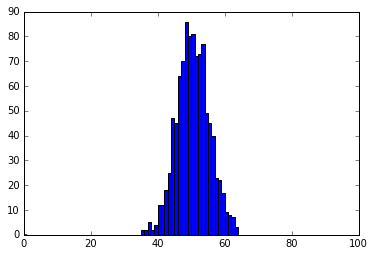
\includegraphics[height=7cm,keepaspectratio=true]{./pe/distBin01.png}
 % distBin01.png: 0x0 pixel, 300dpi, 0.00x0.00 cm, bb=
 \label{distBin01}
\end{figure}


\section{Distribución Normal}

 Una de las distribuciones de probabilidad continua más importantes es la \emph{distribución normal}, también llamada \emph{distribución gaussiana,} que se define mediante la función de densidad
 \begin{align}
  \label{eq:7.3_}
  f_{a,b}(x)=\dfrac{1}{\sqrt{2\pi}}e^{-\frac{1}{2}\frac{(x-a)^{2}}{b^{2}}}
 \end{align}
donde $a,b$ son parámetros específicos para cada v.a. $X.$

{Propiedades de la distribución normal}
 Si la v.a. $X$ tiene la función de densidad dada por \eqref{eq:7.3_}, con parámetros $a,b$ entonces
 \begin{align}
  a = \mu_{X}\\
  b = \s_{X}
 \end{align}



 Si una variable aleatoria normal $X$ tiene función de densidad
  \begin{align}
  \label{eq:7.3_}
  f(x)=\dfrac{1}{\sqrt{2\pi}}e^{-\frac{1}{2}\frac{(x-\mu)^{2}}{\s^{2}}},
 \end{align}
 escribiremos $X\sim N(\mu, \s^{2}).$


{Variable aleatoria normalizada}
 \begin{align}
  \label{van}
  Z = \dfrac{X-\mu}{\s}\\
  \mu_{Z}=0 \\
  \s_{Z}=1
 \end{align}


{Forma Estándar}
 \begin{align}
  \label{eq:7.4}
  f(z)=\dfrac{1}{\sqrt{2\pi}}e^{-\frac{1}{2}z^{2}}
 \end{align}


En este caso, diremos que $Z$ está \emph{normalmente distribuida.}


[fragile, allowframebreaks]{distribucionNormal.py}
 \begin{verbatim}
import scipy.integrate as integrate
import numpy as np
import matplotlib.pyplot as plt
from matplotlib.patches import Polygon

def fn(x,m=0,s=1):
    return np.exp(-(x-m)**2/(2*s**2))/(s*np.sqrt(2*np.pi))
x1 = np.arange(-4,4,0.1)
plt.plot(x1, fn(x1))
plt.show()

for s in np.arange(1,4+1):
    result = integrate.quad(lambda x:fn(x),-s,s)
    print result

for s in np.arange(1,4+1):
    result = integrate.quad(lambda x:fn(x),-s,s)

    a, b = -s, s  # integral limits
    x = np.arange(-4,4,0.01)
    y = fn(x)

    fig, ax = plt.subplots()
    plt.plot(x, y, 'r', linewidth=2)
    plt.ylim(ymin=0)

    # Make the shaded region
    ix = np.linspace(a, b)
    iy = fn(ix)
    verts = [(a, 0)] + list(zip(ix, iy)) + [(b, 0)]
    poly = Polygon(verts, facecolor='0.9', edgecolor='0.5')
    ax.add_patch(poly)

    ax.set_xticks((a, b))
    ax.set_xticklabels(('$-\sigma$', '$\sigma$'))
    ax.set_yticks([])

    plt.show()
    print result
 \end{verbatim}


[fragile]
 \begin{figure}
 \centering
 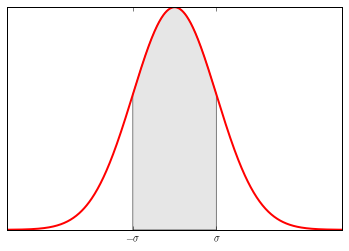
\includegraphics[height=5cm,keepaspectratio=true]{./pe/norm1.png}
 % norm1.png: 0x0 pixel, 300dpi, 0.00x0.00 cm, bb=
 \label{fig:norm1}
\end{figure}
\begin{verbatim}
 #(0.682689492137086, 7.579375928402476e-15)
\end{verbatim}


[fragile]
 \begin{figure}
 \centering
 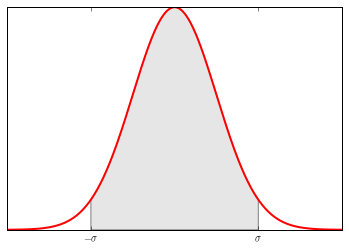
\includegraphics[height=5cm,keepaspectratio=true]{./pe/norm2.png}
 % norm1.png: 0x0 pixel, 300dpi, 0.00x0.00 cm, bb=
 \label{fig:norm2}
\end{figure}
\begin{verbatim}
 #(0.9544997361036417, 1.8403548653972355e-11)
\end{verbatim}


[fragile]
 \begin{figure}
 \centering
 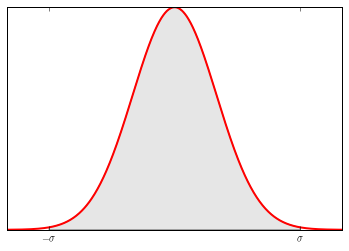
\includegraphics[height=5cm,keepaspectratio=true]{./pe/norm3.png}
 % norm1.png: 0x0 pixel, 300dpi, 0.00x0.00 cm, bb=
 \label{fig:norm3}
\end{figure}
\begin{verbatim}
 #(0.9973002039367399, 1.1072256503105314e-14)
\end{verbatim}


[fragile]
 \begin{figure}
 \centering
 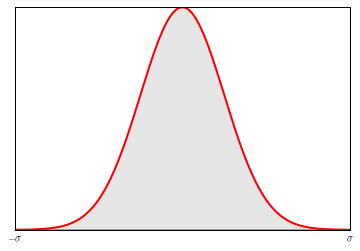
\includegraphics[height=5cm,keepaspectratio=true]{./pe/norm4.png}
 % norm1.png: 0x0 pixel, 300dpi, 0.00x0.00 cm, bb=
 \label{fig:norm4}
\end{figure}
\begin{verbatim}
 #(0.9999366575163339, 4.838904125482879e-12)
\end{verbatim}


[fragile, allowframebreaks]{normalCDF.py}
 \begin{verbatim}
from scipy import stats
import numpy as np
import matplotlib.pyplot as plt

mu = 3.5
sigma = 0.76
nd = stats.norm(mu, sigma)

x = np.arange(mu - 4*sigma,mu + 4*sigma,0.01)
y = nd.cdf(x)

fig, ax = plt.subplots()
plt.plot(x, y, 'r', linewidth=2)
plt.ylim(ymin=0)

for k in range(1,5):
    print nd.cdf(mu+k*sigma)-nd.cdf(mu-k*sigma)

#0.682689492137
#0.954499736104
#0.997300203937
#0.999936657516
 \end{verbatim}
\begin{center}
 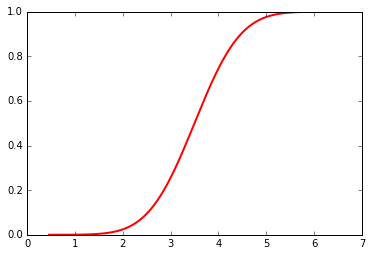
\includegraphics[height=5cm,keepaspectratio=true]{./pe/normCDF.png}
 % normCDF.png: 0x0 pixel, 300dpi, 0.00x0.00 cm, bb=
\end{center}



\section{Relación entre las distribuciones binomial y normal}

 Si $N\sim \infty, p,q>>0,$ y $X$ es un distribución binomial con parámetros $N,p$ entonces
 \begin{align}
  \dfrac{X-Np}{\sqrt{Npq}} \sim N(0,1).
 \end{align}



 \begin{ejemplo}
  \label{exmp:7.5}
  Consideremos el experimento de lanzar 16 veces una moneda. Repitamos 1,000,000 dicho experimento. Compruebe que dicho experimento se puede modelar por una variable aleatoria con distribución $N(\mu=8,\sigma^{2}=4)$
 \end{ejemplo}


[fragile, allowframebreaks]{relBinomNormal.py}
 \begin{verbatim}
import numpy as np
import matplotlib.pyplot as plt

def fn(x,m=0,s=1):
    C = 1/(s*np.sqrt(2*np.pi))
    return C*np.exp(-(x-m)**2/(2*s**2))

N,p=30, 0.5
R = 1000000
q=1-p
mB = N*p
sB = np.sqrt(N*p*q)
X = np.random.binomial(N,p,R)
myBins = np.arange(-0.5,N+0.5,1)
plt.hist(X, bins = myBins)
x = np.arange(mB-4*sB,mB+4*sB+0.1,0.1)
y = R*fn(x, m=mB, s=sB)
plt.plot(x,y,lw=2)
plt.ylim(ymin=0)
plt.show()
 \end{verbatim}
\begin{center}
 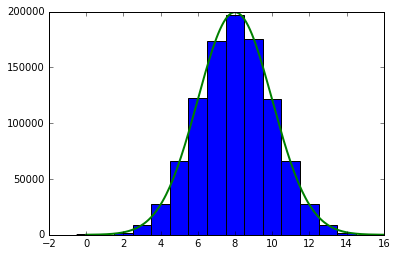
\includegraphics[height=5cm]{./pe/relBinNorm.png}
 % relBinNorm.png: 0x0 pixel, 300dpi, 0.00x0.00 cm, bb=
\end{center}



\section{La Distribución de Poisson}
{Distribución de Poisson} Diremos que una variable aleatoria \emph{discreta} $X$ tiene distribución de Poisson si su función de probabilidad está dada por:
 \begin{align}
  \label{eq:7.5}
  f(n)=\dfrac{\lam^{n}e^{-\lam}}{n!}, \; n=0,1,2,...
 \end{align}


En este caso, $\mu_{X}=\s^{2}=\lam.$


\begin{quote}
 En teoría de probabilidad y estadística, la distribución de Poisson es una distribución de probabilidad discreta que expresa, a partir de una frecuencia de ocurrencia media, la probabilidad de que ocurra un determinado número de eventos durante cierto período de tiempo. Concretamente, se especializa en la probabilidad de ocurrencia de sucesos con probabilidades muy pequeñas, o sucesos raros.
\end{quote}

\href{https://es.wikipedia.org/wiki/Distribuci\%C3\%B3n_de_Poisson}{Wikipedia: Distribución de Poisson}


 \begin{ejemplo}
  \label{exmp:7.6}
  El número de personas por día que llegan a una sala de urgencias tiene una distribución de Poisson con media 5. Hallar la probabilidad de que cuando mucho lleguen tres por día y la probabilidad de que por lo menos lleguen 8 personas por día.
 \end{ejemplo}




[fragile, allowframebreaks]{distPoisson.py}
 \begin{verbatim}
from scipy import stats
import numpy as np
import matplotlib.pyplot as plt

def f(x, mu=1):
    return stats.poisson.pmf(x, mu)

def F(x, mu=1):
    return stats.poisson.cdf(x, mu)

x1 = np.arange(0,100+1)
plt.plot(x1, f(x1, mu=5), 'bo')
plt.show()

s = np.random.poisson(5,365)
M = np.max(s)
myBins = np.arange(0,M+1)
plt.hist(s, bins = myBins)
plt.show()

print F(3, mu=5)
print 1 - F(7, mu=5)

for k in range(12+1):
    print k, F(k, 5)
"""
0 0.00673794699909
1 0.0404276819945
2 0.124652019483
3 0.265025915297
4 0.440493285065
5 0.615960654833
6 0.762183462973
7 0.86662832593
8 0.931906365278
9 0.968171942694
10 0.986304731402
11 0.994546908087
12 0.997981148373
"""
 \end{verbatim}



 \begin{figure}
 \centering
 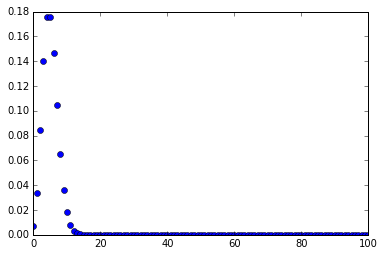
\includegraphics[height=7cm,keepaspectratio=true]{./pe/distPoisson0.png}
 % distPoisson0.png: 0x0 pixel, 300dpi, 0.00x0.00 cm, bb=
 \caption{Distribución de Poisson}
\end{figure}




\begin{figure}
 \centering
 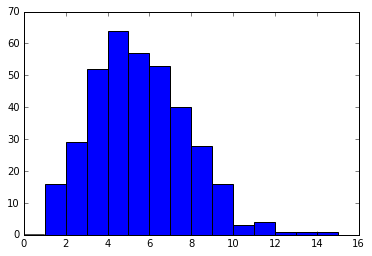
\includegraphics[height=7cm,keepaspectratio=true]{./pe/distPoisson1.png}
 % distPoisson1.png: 0x0 pixel, 300dpi, 0.00x0.00 cm, bb=
 \caption{Histograma de pacientes en sala de urgencias durante un año con media $\lam=5$}
 \label{fig:distPoisson1}
\end{figure}



\section{Relación entre las Distribuciones Binomiales y de Poisson}

 Si en la función de probabilidad binomial, $N$ es muy grande pero $p \approx 0,$ esto modela un \emph{evento raro}.  En la práctica esto significa $N>>50, Np<<5.$ 

 En este caso, la distribución Binomial con parámetros $N,p$ se aproxima a una Poisson con parámetro $\lam = Np.$

[fragile, allowframebreaks]{relBinomPoisson.py}
 \begin{verbatim}
from scipy import stats
import numpy as np
import matplotlib.pyplot as plt
import matplotlib as mpl

mpl.style.use("ggplot")

fig, ax = plt.subplots(1, 1)

def fP(x, mu=1):
    return stats.poisson.pmf(x, mu)

def fB(x, N=30, p=0.5):
    return stats.binom(N,p).pmf(x)

N_=50
p_=5./N_
mu_ = N_*p_
x1 = np.arange(0,20+1)
ax.plot(x1, fP(x1, mu=mu_), 'bo', label="Poisson")
ax.plot(x1, fB(x1, N=N_, p=p_), 'ro', label="Binomial")
legend = ax.legend(loc='upper center', shadow=True)
plt.show()

 \end{verbatim}



 \begin{figure}
 \centering
 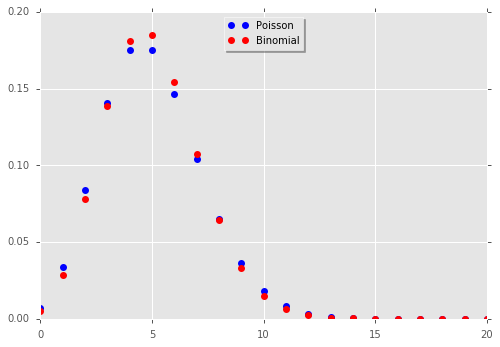
\includegraphics[height=7cm]{./pe/binVsPoi.png}
 % binVsPoi.png: 0x0 pixel, 300dpi, 0.00x0.00 cm, bb=
 \caption{Comparación entre distribuciones Binomial y Poisson para eventos raros.}
\end{figure}



\section{Distribución multinomial}

 Si los eventos $E_{1},...,E_{k}$ pueden ocurrir con probabilidades $p_{1},...,p_{k}$ respectivamente, entonces la probabilidad de que ocurran $X_{1},...,x_{k}$ veces respectivamente esta dado por la \emph{distribución multinomial}
 \begin{align}
  \label{eq:7.6}
  f\left( x_{1},...,x_{2} \right)=
  \dfrac{x_{1}+...+x_{k}}{x_{1}!...x_{k}!}p_{1}^{x_{1}}\cdots p_{k}^{x_{k}}.
 \end{align}



 \begin{ejemplo}
  \label{exmp:7.7}
Si un dado se lanza 12 veces, encontrar la probabilidad de obtener cada uno de los números $1,2,3,4,5,6$ exactamente dos veces.
 \end{ejemplo}



\section{Problemas Resueltos}
{Percentil}
 Diremos que $x=P_{q}$ es el percentil $q, \; 0\leq q \leq 100$ de la distribución $F(x)$ si $F(P_{q})=q\%.$  En el caso de que $q$ sea un valor realizable de $F(x),$ podemos \emph{``despejar''}
 \begin{align}
  P_{q}=F^{-1}\left( \dfrac{q}{100} \right).
 \end{align}
 A tal función se le llama \emph{distribución inversa.}


{Cuartiles}
 En la literatura se definen conceptos similares. Por ejemplo, el primer \emph{cuartil} corresponde al percentil $25;$ el segundo cuartil al percentil $50;$ y así sucesivamente.

{Combinaciones}
 \begin{ejemplo}
  \label{sol:7.1}
  Encuentre
  \begin{enumerate}
   \item $5!$
   \item $\comb{8}{3}$
  \end{enumerate}
  utilizando \texttt{Python.}
 \end{ejemplo}


[fragile, allowframebreaks]{combinaciones.py}
 \begin{verbatim}
import math
import scipy.special

print math.factorial(5)
print scipy.special.binom(8,3)
 \end{verbatim}




{Distribución Binomial}
 \begin{ejemplo}
  \label{sol:7.2}
  Supóngase que $15\%$ de la población es zurda. Encontrar la probabilidad de que en un grupo de 50 individuos haya:
  \begin{enumerate}
   \item cuando mucho 10 zurdos; 
   \item por lo menos 5 zurdos; 
   \item entre 3 y 6 zurdos; 
   \item exactamente 5 zurdos.
  \end{enumerate}

 \end{ejemplo}


[fragile, allowframebreaks]{solvedBinom.py}
 \begin{verbatim}
from scipy import stats

#7.2 N=50, p=15%
def f(x):
    return stats.binom(50,.15).pmf(x)
def F(x):
    return stats.binom(50,.15).cdf(x)
#(a) P(X<=10)
print sum([f(x) for x in range(0,10+1)])
##0.8800826828
print F(10)
##0.8800826828
#(b) P(X>=5)
print 1-sum([f(x) for x in range(0,4+1)])
##0.887894791945
print 1-F(4)
##0.887894791945
#(c) P(3<=X<=6)
print sum([f(x) for x in range(3,6+1)])
##0.3471108697
print F(6)-F(2)
##0.3471108697
#(d) P(X=5)
print f(5)
##0.3471108697
 \end{verbatim}



{Distribución Normal}
 \begin{ejemplo}
  \label{sol:7.14}
  En un examen final de matemáticas, la media fue 72 y la desviación estándar fue 15. Determinar las puntuaciones estándar de los estudiantes que obtuvieron:
  \begin{enumerate}
   \item $60$;
   \item $93$;
   \item $72$.
  \end{enumerate}

 \end{ejemplo}



 \begin{ejemplo}
  \label{sol:7.15}
  Con los datos del problema \ref{sol:7.14}, encontrar las calificaciones que corresponden a las siguientes puntuaciones estándar:
  \begin{enumerate}
   \item $-1$;
   \item $1.6$.
  \end{enumerate}

 \end{ejemplo}



 \begin{ejemplo}
  \label{sol:7.16}
  Supóngase que la cantidad de juegos en que participan los beisbolistas de la liga mayor durante su carrera se distribuye normalmente con media de $1500$ juegos y desviación estándar $350$ juegos. Emplear \texttt{Python} para responder las siguientes preguntas:
  \begin{enumerate}
   \item ¿Qué porcentaje participa en menos de 750 juegos?;
   \item ¿qué porcentaje participa en más de 2000 juegos?;
   \item encontrar el \emph{percentil} $90$ de la cantidad de juegos en los que participan en su carrera.
  \end{enumerate}

 \end{ejemplo}


[fragile, allowframebreaks]{solvedNorm.py}
 \begin{verbatim}
from scipy import stats

mu = 1500
sigma = 350
nd = stats.norm(mu, sigma)

def F(x):
    return nd.cdf(x)

#a
print F(750)
##0.3471108697

#b
print 1-F(2000)
##0.0765637255098

def inverseF(x):
    return nd.ppf(x)
#c
print inverseF(.90)
##1948.54304794
 \end{verbatim}


{Eventos raros}
\begin{ejemplo}
\label{sol:7.28}
  Si la probabilidad de que un individuo tenga una reacción adversa por la inyección de determinado suero es $0.001,$ determinar la probabilidad de que de 2000 individuos:
 \begin{enumerate}
  \item exactamente 3;
  \item más de 2
 \end{enumerate}
sufran una reacción adversa.
\end{ejemplo}


[fragile, allowframebreaks]{eventosRaros.py}
 \begin{verbatim}
from scipy import stats
#7.28
#a
N = 2000
p = 0.001
print stats.binom(N,p).pmf(3)
##0.180537328032
print stats.poisson(N*p).pmf(3)
##0.180447044315
#(b)
print 1-stats.binom(N,p).cdf(2)
##0.32332356124
print 1-stats.poisson(N*p).cdf(2)
##0.323323583817
 \end{verbatim}


